\documentclass[12pt, a4paper]{article}

% --- PACOTES ---
\usepackage[utf8]{inputenc}
\usepackage[T1]{fontenc}
\usepackage[portuguese]{babel}
\usepackage{geometry}
\usepackage{graphicx}
\usepackage[dvipsnames]{xcolor} % Adicionado para suporte avançado de cores
\usepackage{amsmath}
\usepackage{hyperref}
\usepackage{booktabs} 
\usepackage{listings} 
\usepackage{float}    

% --- CONFIGURAÇÕES ---

% Geometria da página
\geometry{a4paper, margin=2.5cm}

% Configurações de links do hyperref
\hypersetup{
    colorlinks=true,
    linkcolor=blue,
    filecolor=magenta,      
    urlcolor=cyan,
    pdftitle={Relatório do Projeto: Odd-Even Transposition Sort Paralelo},
    pdfpagemode=FullScreen,
}

% Configurações para listagens de código (listings)
\lstset{
    language=C,
    basicstyle=\ttfamily\small,
    keywordstyle=\color{blue},
    commentstyle=\color{green!50!black},
    stringstyle=\color{red},
    breakatwhitespace=false,
    breaklines=true,
    captionpos=b,
    keepspaces=true,
    numbers=left,
    numbersep=5pt,
    showspaces=false,
    showstringspaces=false,
    showtabs=false,
    tabsize=2,
    frame=single,
    rulecolor=\color{black!30},
    title=\lstname,
}

% --- DOCUMENTO ---

\title{
    \textbf{Relatório do Projeto} \\
    \vspace{0.2cm}
    \large Odd-Even Transposition Sort Paralelo com OpenMP e MPI \\
    \large Computação de Alto Desempenho - UFRJ
}
\author{
    Aluno: Guilherme Oliveira Rolim Silva \\
    DRE: 122076696
}
\date{\today}

\begin{document}

\maketitle
\thispagestyle{empty}

\begin{center}
    \textbf{Link para o repositório:} \href{https://github.com/rolim520/Odd-Even-Transposition-Sort-Paralelo}{https://github.com/rolim520/Odd-Even-Transposition-Sort-Paralelo}
\end{center}

\section{Introdução}


O trabalho tem como objetivo explorar a paralelização do algoritmo de ordenação \textit{Odd-Even Transposition Sort}. Este algoritmo de ordenação se destaca por sua estrutura inerentemente paralelizável. O algoritmo opera em fases alternadas: uma fase "par" (even), onde são realizadas comparações entre elementos em posições de índice par e seus sucessores (i, i+1), e uma fase "ímpar" (odd), que faz o mesmo para elementos em posições de índice ímpar e seus sucessores. Após $n$ fases, onde $n$ é o número de elementos, o array está garantidamente ordenado.

O objetivo principal deste projeto é implementar e analisar o desempenho de duas versões paralelas deste algoritmo: uma utilizando o paradigma de memória compartilhada com \textbf{OpenMP} e outra utilizando o paradigma de troca de mensagens com \textbf{MPI (Message Passing Interface)}. O desempenho das versões paralelas será comparado com uma implementação serial de referência para avaliar métricas como \textit{speedup}, eficiência e \textit{overhead}.

\section{Metodologia}

Nesta seção, descrevemos as três implementações desenvolvidas (Serial, OpenMP e MPI) e o ambiente utilizado para a execução e análise dos testes.

\subsection{Ambiente de Teste}
Os experimentos foram conduzidos em um ambiente com as seguintes especificações (exemplo):
\begin{itemize}
    \item \textbf{Processador:} AMD Ryzen 5 5600X 6-Core Processor (12 threads)
    \item \textbf{Memória RAM:} 32 GB DDR4
    \item \textbf{Sistema Operacional:} Fedora Linux
    \item \textbf{Compilador (Serial e OpenMP):} GCC
    \item \textbf{Compilador (MPI):} MPICC (wrapper do Open MPI)
\end{itemize}
Os tempos de execução foram medidos utilizando \texttt{clock\_gettime(CLOCK\_MONOTONIC)} para a versão serial e \texttt{omp\_get\_wtime()} para a versão OpenMP, garantindo medições de alta precisão. Na versão MPI, o tempo foi medido com \texttt{MPI\_Wtime()}.

\subsection{Implementação Serial}
A implementação serial serve como linha de base para nossos comparativos de desempenho. O algoritmo executa um laço principal $n$ vezes (o número de fases). Dentro de cada fase, ele verifica se a fase é par ou ímpar e, em seguida, percorre o array realizando as comparações e trocas necessárias.

\begin{lstlisting}[caption={Trecho do laço principal da versão serial.}, label=lst:serial]
void odd_even_sort_serial(int arr[], int n) {
    int phase, i;
    for (phase = 0; phase < n; phase++) {
        if (phase % 2 == 0) { // Fase par
            for (i = 1; i < n; i += 2) {
                if (arr[i - 1] > arr[i]) {
                    swap(&arr[i - 1], &arr[i]);
                }
            }
        } else { // Fase impar
            for (i = 1; i < n - 1; i += 2) {
                if (arr[i] > arr[i + 1]) {
                    swap(&arr[i], &arr[i + 1]);
                }
            }
        }
    }
}
\end{lstlisting}

\subsection{Implementação com OpenMP}
A versão com OpenMP paraleliza os laços internos de cada fase (par e ímpar) usando a diretiva \texttt{\#pragma omp for}. As threads compartilham o array e trabalham em diferentes partes dele simultaneamente. Foram implementadas funções com cada uma das 3 schedules disponiveis (static, dynamic e guided). Abaixo está a implementação com o schedule \texttt{static}.


\begin{lstlisting}[caption={Paralelização de uma fase com OpenMP.}, label=lst:openmp]
#pragma omp parallel num_threads(num_threads) default(none) shared(arr, n) private(phase, i)
    {
        for (phase = 0; phase < n; phase++) {
            if (phase % 2 == 0) { // Fase Par
                #pragma omp for schedule(static)
                for (i = 1; i < n; i += 2) {
                    if (arr[i - 1] > arr[i]) {
                        swap(&arr[i - 1], &arr[i]);
                    }
                }
            } else { // Fase Impar
                #pragma omp for schedule(static)
                for (i = 1; i < n - 1; i += 2) {
                    if (arr[i] > arr[i + 1]) {
                        swap(&arr[i], &arr[i + 1]);
                    }
                }
            }
        }
    }
\end{lstlisting}

\subsection{Implementação com MPI}
A implementação com MPI adota um paralelismo de dados, onde o array é distribuído entre os processos. A lógica replica a estrutura de fases do algoritmo original de forma distribuída:
\begin{enumerate}
    \item \textbf{Distribuição de Dados:} O processo raiz distribui porções do array para todos os outros processos usando \texttt{MPI\_Scatterv}, que permite a distribuição de blocos de tamanhos desiguais, relevante caso o array não seja perfeitamente divisível pelo número de processos.
    \item \textbf{Loop de Fases Sincronizado:} O loop principal executa $n$ vezes, correspondendo às $n$ fases do algoritmo. Em cada fase, todos os processos executam simultaneamente a mesma etapa (par ou ímpar) em seu sub-array local. Isso é feito pela função \texttt{single\_phase\_odd\_even}.
    \item \textbf{Comunicação de Fronteiras:} Após a etapa de computação local, os processos precisam comparar e, se necessário, trocar os elementos nas fronteiras de seus sub-arrays. A comunicação é feita com \texttt{MPI\_Sendrecv} para evitar deadlocks. A lógica de parceria (par com ímpar) garante que as comparações corretas do algoritmo global sejam mantidas.
    \item \textbf{Coleta de Resultados:} Ao final de todas as fases, \texttt{MPI\_Allgatherv} é usado para reunir os sub-arrays ordenados de todos os processos. O resultado é que cada processo recebe o array global totalmente ordenado.
\end{enumerate}

O algoritmo foi implementado com a troca das fronteiras de cada array local com seus vizinhos, de acordo como foi especificado no enunciado do trabalho. Entretanto, desse modo a comunicação está sendo executada a cada iteração de fase, o que possivelmente foi o fator determinante no baixo desempenho do algoritmo para tamanhos de array menores. Apesar disso, optou-se por se manter fiel ao enunciado do trabalho. O trecho de código abaixo ilustra a lógica de comunicação e comparação de fronteiras.

\begin{lstlisting}[caption={Lógica de comunicação de fronteira na implementação MPI.}, label=lst:mpi]
// ... dentro do loop de fases ...
// Determina o processo parceiro para a troca
int partner;
if ((phase % 2) == 0) {
    partner = (rank % 2 == 0) ? rank + 1 : rank - 1;
} else {
    partner = (rank % 2 != 0) ? rank + 1 : rank - 1;
}

if (partner >= 0 && partner < size) {
    // Determina qual valor enviar (primeiro ou ultimo elemento local)
    int send_val = (rank < partner) ? local_arr[local_n - 1] : local_arr[0];
    int recv_val;
    
    // Envia e recebe o valor da fronteira simultaneamente
    MPI_Sendrecv(&send_val, 1, MPI_INT, partner, 0,
                 &recv_val, 1, MPI_INT, partner, 0,
                 MPI_COMM_WORLD, MPI_STATUS_IGNORE);

    // Compara e atualiza o valor da fronteira se necessario
    if (rank < partner) { // Compara ultimo local com primeiro do vizinho
        if (send_val > recv_val) local_arr[local_n - 1] = recv_val;
    } else { // Compara primeiro local com ultimo do vizinho
        if (recv_val > send_val) local_arr[0] = recv_val;
    }
}
\end{lstlisting}

\subsection{Métricas de Desempenho}
Para avaliar a performance das implementações paralelas, foram definidas e calculadas as seguintes métricas, exportadas para arquivos CSV ao final de cada execução.

\begin{itemize}
    \item \textbf{Tempo Serial ($T_s$):} O tempo de parede (wall-clock time) para executar a versão sequencial do algoritmo. Serve como linha de base para os cálculos de aceleração.
    
    \item \textbf{Tempo Paralelo ($T_p$):} O tempo de parede da versão paralela. Foi calculado como o tempo máximo entre todos os processos (\texttt{MPI\_MAX}), pois o tempo total é determinado pelo processo que demora mais para terminar.
    
    \item \textbf{Speedup ($S$):} Mede o ganho de desempenho da versão paralela em relação à serial. É calculado pela razão $S = T_s / T_p$. Um speedup de $k$ significa que a versão paralela foi $k$ vezes mais rápida.
    
    \item \textbf{Eficiência ($E$):} Mede quão bem os recursos de processamento foram aproveitados. É calculada como $E = S / P$, onde $P$ é o número de processos/threads. Uma eficiência de 1 (ou 100\%) é ideal, indicando que todos os processadores foram usados de forma produtiva durante todo o tempo.
    
    \item \textbf{Overhead de Comunicação:} Representa o tempo gasto em atividades que não são computação útil, principalmente a troca de mensagens em MPI. Foi calculado de duas formas:
    \begin{itemize}
        \item \textbf{Tempo de Comunicação (soma):} Soma do tempo gasto em chamadas \texttt{MPI\_Sendrecv} por todos os processos.
        \item \textbf{Overhead Relativo (\%):} Percentual do tempo total (soma de computação e comunicação de todos os processos) que foi gasto apenas com comunicação. Esta métrica é útil para entender o impacto da comunicação na performance geral.
    \end{itemize}
\end{itemize}


\subsection{Automação da Coleta de Dados e Geração de Gráficos}
Para garantir a consistência e a reprodutibilidade dos experimentos, o processo de coleta de dados e a criação dos gráficos foram automatizados com o uso de scripts.

\paragraph{Coleta de Dados}
Um script em Shell, \texttt{run\_experiments.sh}, foi desenvolvido para executar sistematicamente as três versões do algoritmo (serial, OpenMP e MPI). O script iterou sobre arrays com tamanhos de 1k, 5k, 10k, 50k e 100k elementos, assim como, para as versões paralelas, sobre 1, 2, 4 e 8 números de threads (OpenMP) e processos (MPI). A saída de cada execução, contendo o tempo de execução e os parâmetros do teste, foi redirecionada e salva em arquivos no formato CSV (\texttt{.csv}) dentro do diretório \texttt{data/}.

\paragraph{Geração de Gráficos}
Após a coleta, um script em Python, \texttt{plot\_graphs.py}, foi utilizado para processar os dados. Utilizando as bibliotecas \texttt{pandas} para a leitura e manipulação dos arquivos CSV e \texttt{matplotlib} para a visualização, o script gerou automaticamente todos os gráficos apresentados na seção de Resultados. Isso inclui os gráficos de tempo de execução, speedup e eficiência, garantindo que as visualizações sejam um reflexo fiel dos dados coletados.

\section{Resultados e Análise}
Nesta seção, apresentamos os resultados obtidos nos experimentos, comparando o desempenho das implementações serial, OpenMP e MPI.



\subsection{Tabelas de Desempenho}
As tabelas a seguir resumem os dados de desempenho obtidos a partir da média de múltiplas execuções.

\begin{table}[H]
\centering
\caption{Análise de desempenho do OpenMP por política de schedule para N=100.000.}
\label{tab:openmp-schedule}
\begin{tabular}{lcccc}
\toprule
\textbf{Schedule} & \textbf{Threads} & \textbf{Tempo (s)} & \textbf{Speedup} & \textbf{Eficiência} \\
\midrule
static            & 2                & 3.3781             & 2.5975           & 1.2988              \\
                  & 4                & 1.3457             & 6.5227           & 1.6307              \\
                  & 8                & 1.1291             & 7.7389           & 0.9674              \\
\midrule
guided            & 2                & 3.9768             & 2.2073           & 1.1036              \\
                  & 4                & 2.5667             & 3.4178           & 0.8544              \\
                  & 8                & 1.6368             & 5.3378           & 0.6672              \\
\midrule
dynamic           & 2                & 124.5843           & 0.0704           & 0.0352              \\
                  & 4                & 110.8358           & 0.0792           & 0.0198              \\
                  & 8                & 96.6977            & 0.0904           & 0.0113              \\
\bottomrule
\end{tabular}
\end{table}

\begin{table}[H]
\centering
\caption{Análise de escalabilidade da implementação MPI (P > 1).}
\label{tab:mpi-all-sizes-filtered}
\begin{tabular}{cccccc}
\toprule
\textbf{Tamanho} & \textbf{Processos} & \textbf{Tempo (s)} & \textbf{Speedup} & \textbf{Eficiência} & \textbf{Overhead (\%)} \\
\midrule
1,000 & 2 & 0.0005 & 1.1903 & 0.5952 & 45.08 \\
 & 4 & 0.0012 & 0.5036 & 0.1259 & 83.11 \\
 & 8 & 0.0015 & 0.4402 & 0.0550 & 90.50 \\
\midrule
5,000 & 2 & 0.0071 & 1.6614 & 0.8307 & 18.43 \\
 & 4 & 0.0056 & 2.1534 & 0.5383 & 46.30 \\
 & 8 & 0.0080 & 1.7363 & 0.2170 & 74.67 \\
\midrule
10,000 & 2 & 0.0250 & 1.7844 & 0.8922 & 11.77 \\
 & 4 & 0.0163 & 2.7237 & 0.6810 & 30.78 \\
 & 8 & 0.0196 & 2.8041 & 0.3505 & 61.30 \\
\midrule
50,000 & 2 & 0.6529 & 2.8441 & 1.4221 & 3.85 \\
 & 4 & 0.3168 & 5.8158 & 1.4539 & 11.14 \\
 & 8 & 0.3007 & 6.5020 & 0.8128 & 36.21 \\
\midrule
100,000 & 2 & 3.7764 & 2.3194 & 1.1597 & 1.93 \\
 & 4 & 1.8673 & 4.7007 & 1.1752 & 21.74 \\
 & 8 & 1.2315 & 7.4138 & 0.9267 & 33.26 \\
\bottomrule
\end{tabular}
\end{table}

\subsection{Análise Gráfica}

\begin{figure}[H]
    \centering
    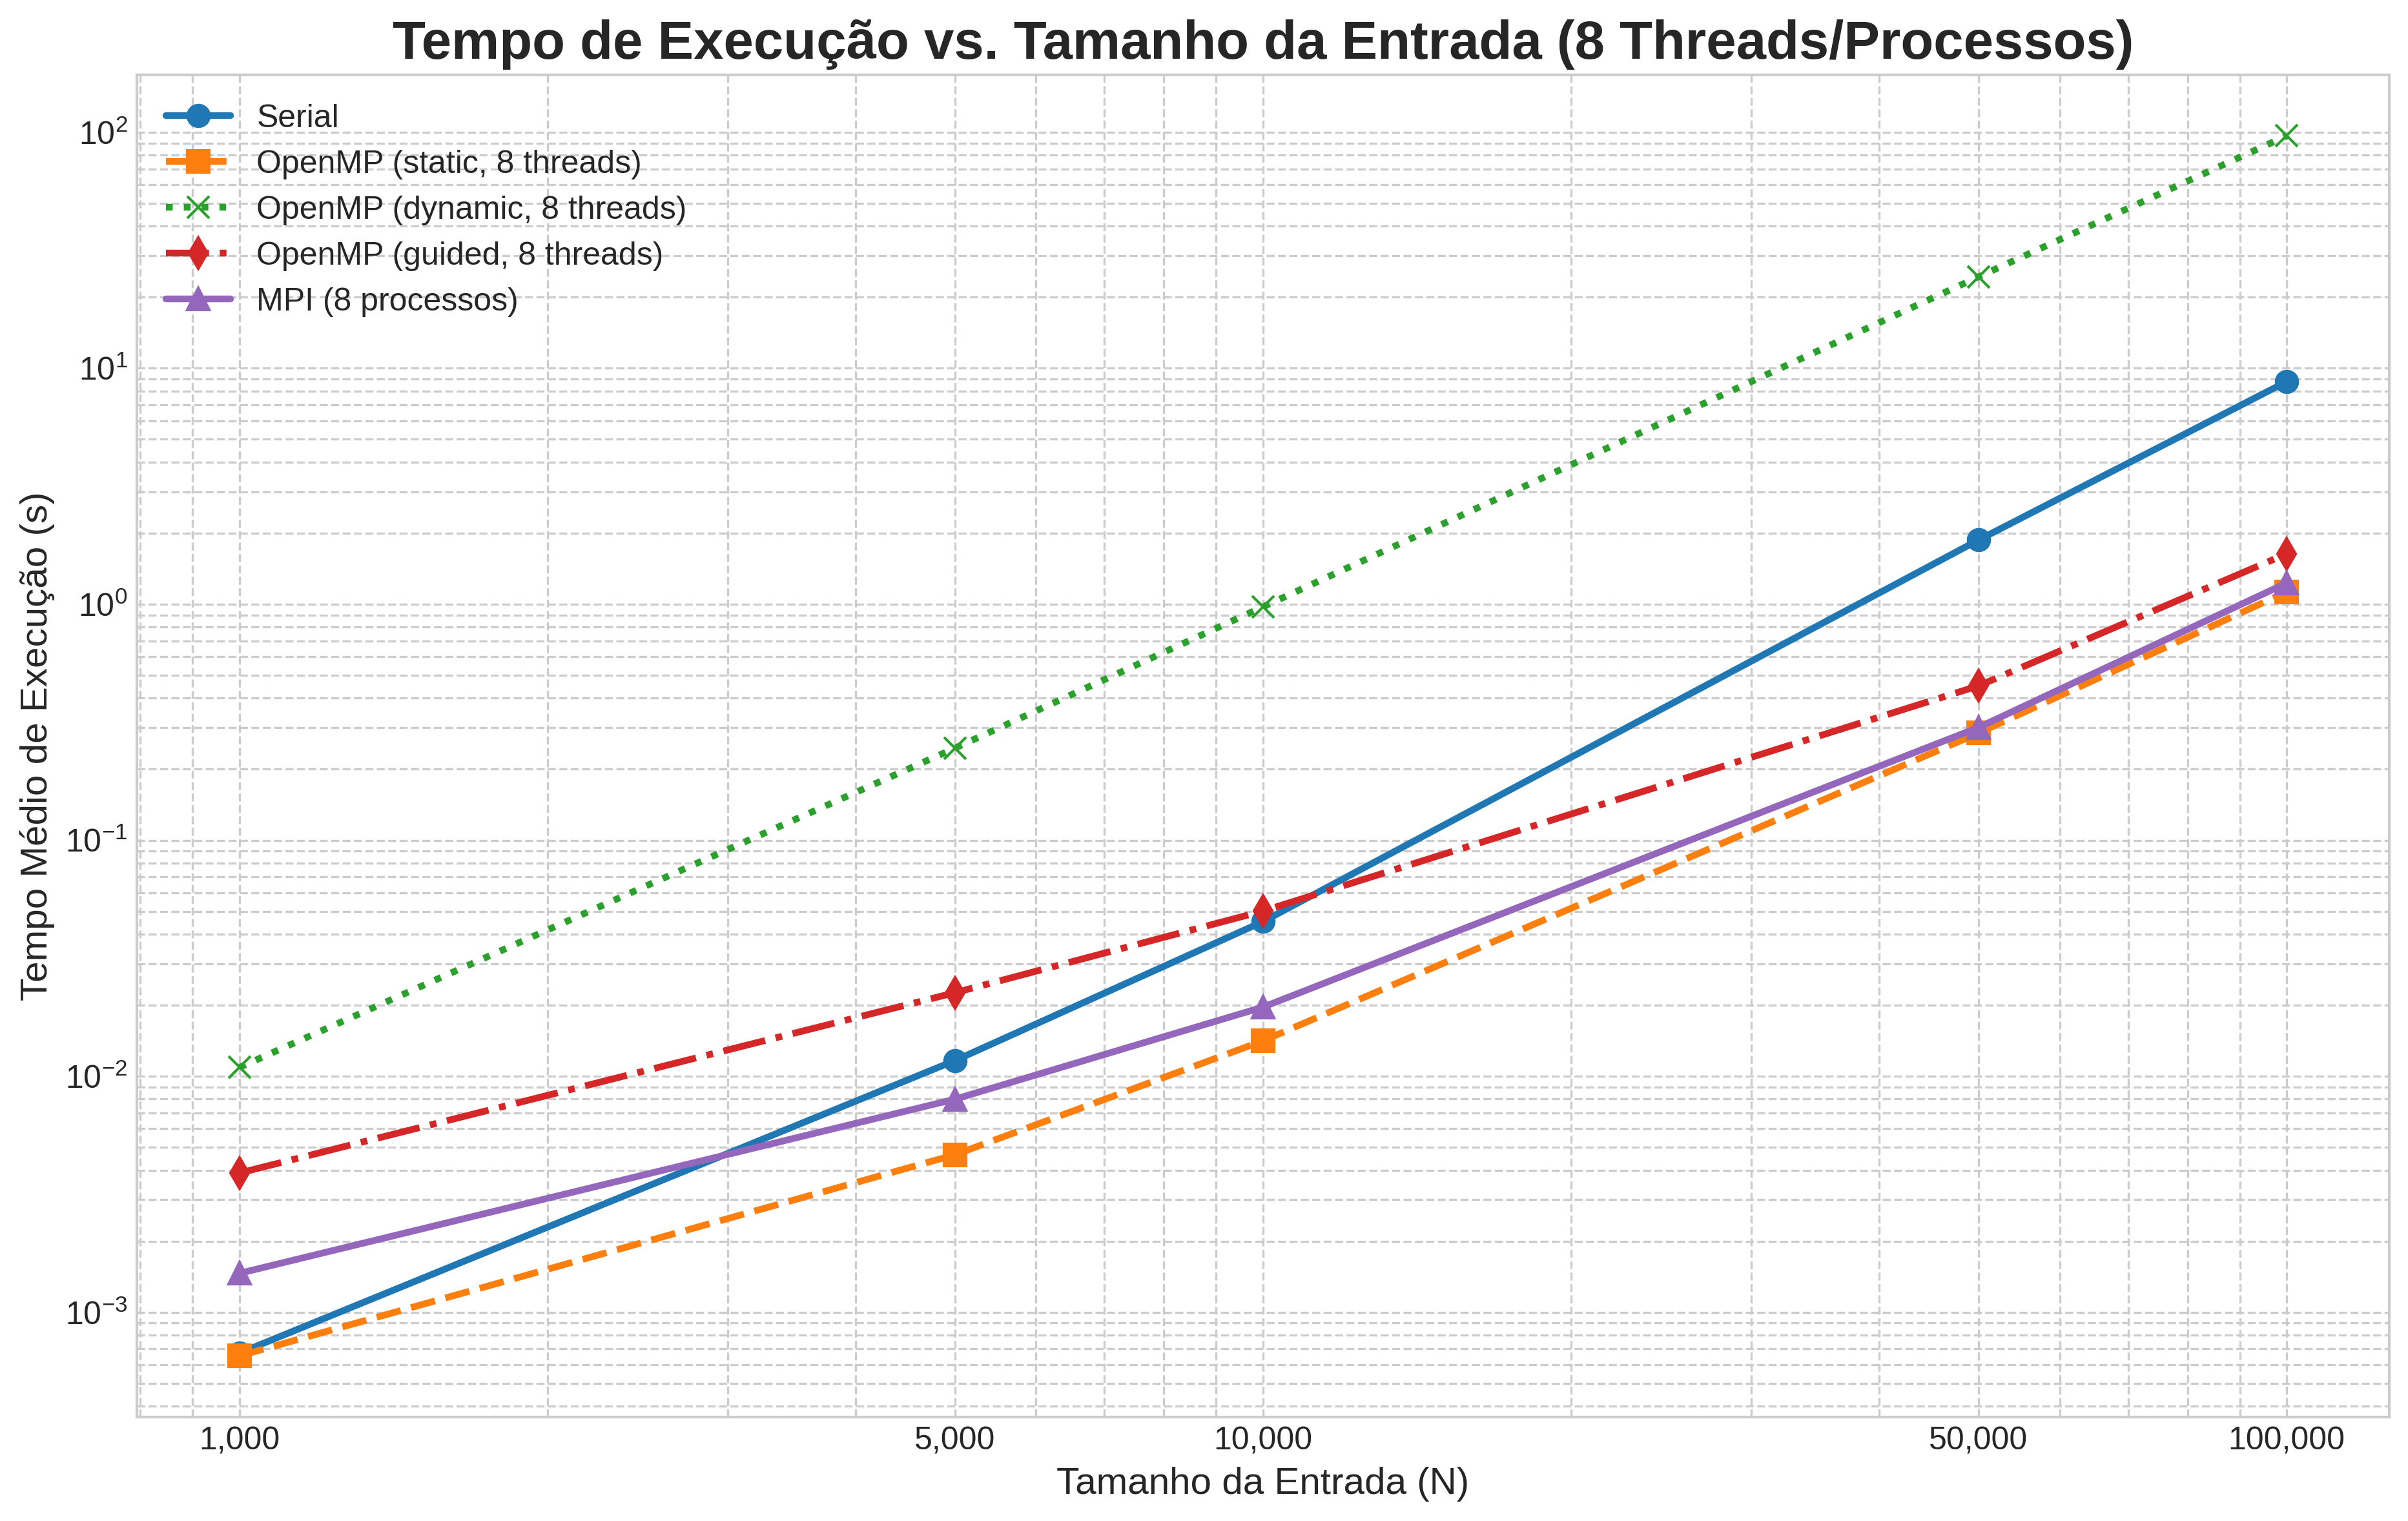
\includegraphics[width=0.9\textwidth]{../graficos/tempo_vs_tamanho_8_threads.png}
    \caption{Tempo vs. Tamanho do Array (8 threads/processos).}
    \label{fig:tempo_vs_tamanho}
\end{figure}

\begin{figure}[H]
    \centering
    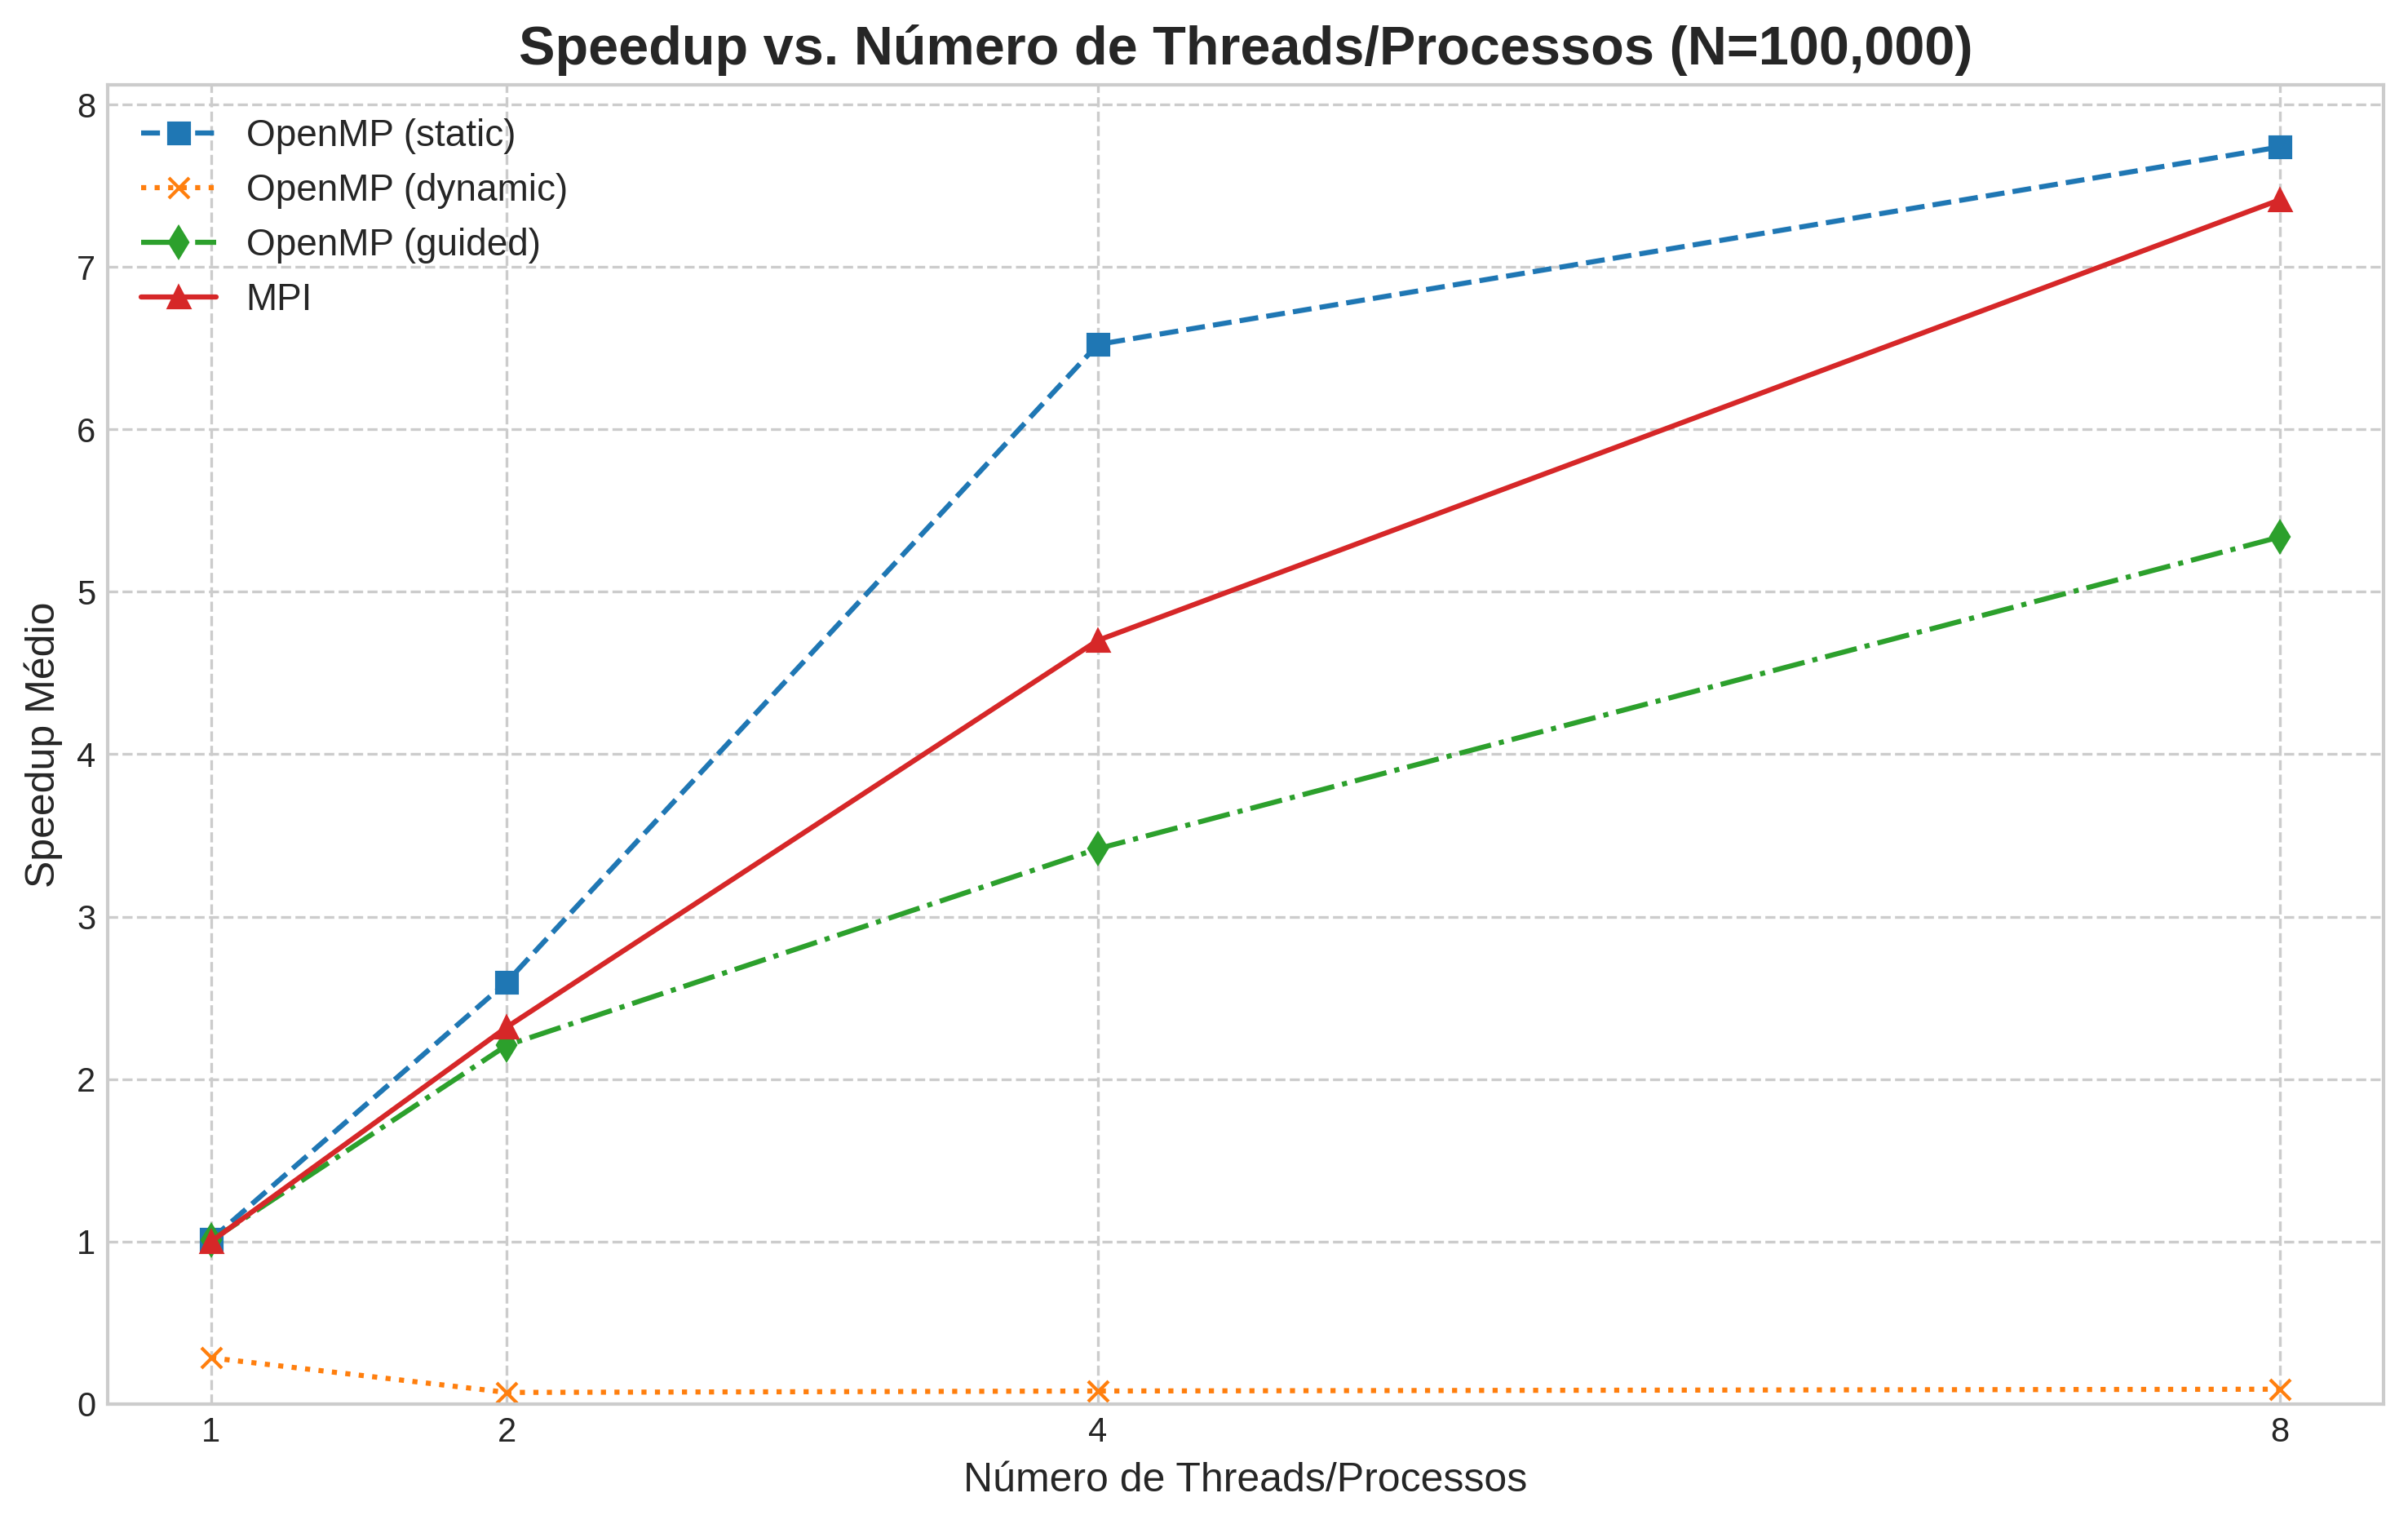
\includegraphics[width=0.9\textwidth]{../graficos/speedup_vs_processos_100000.png}
    \caption{Speedup vs. Número de Processos/Threads ($N=100.000$).}
    \label{fig:speedup}
\end{figure}

\begin{figure}[H]
    \centering
    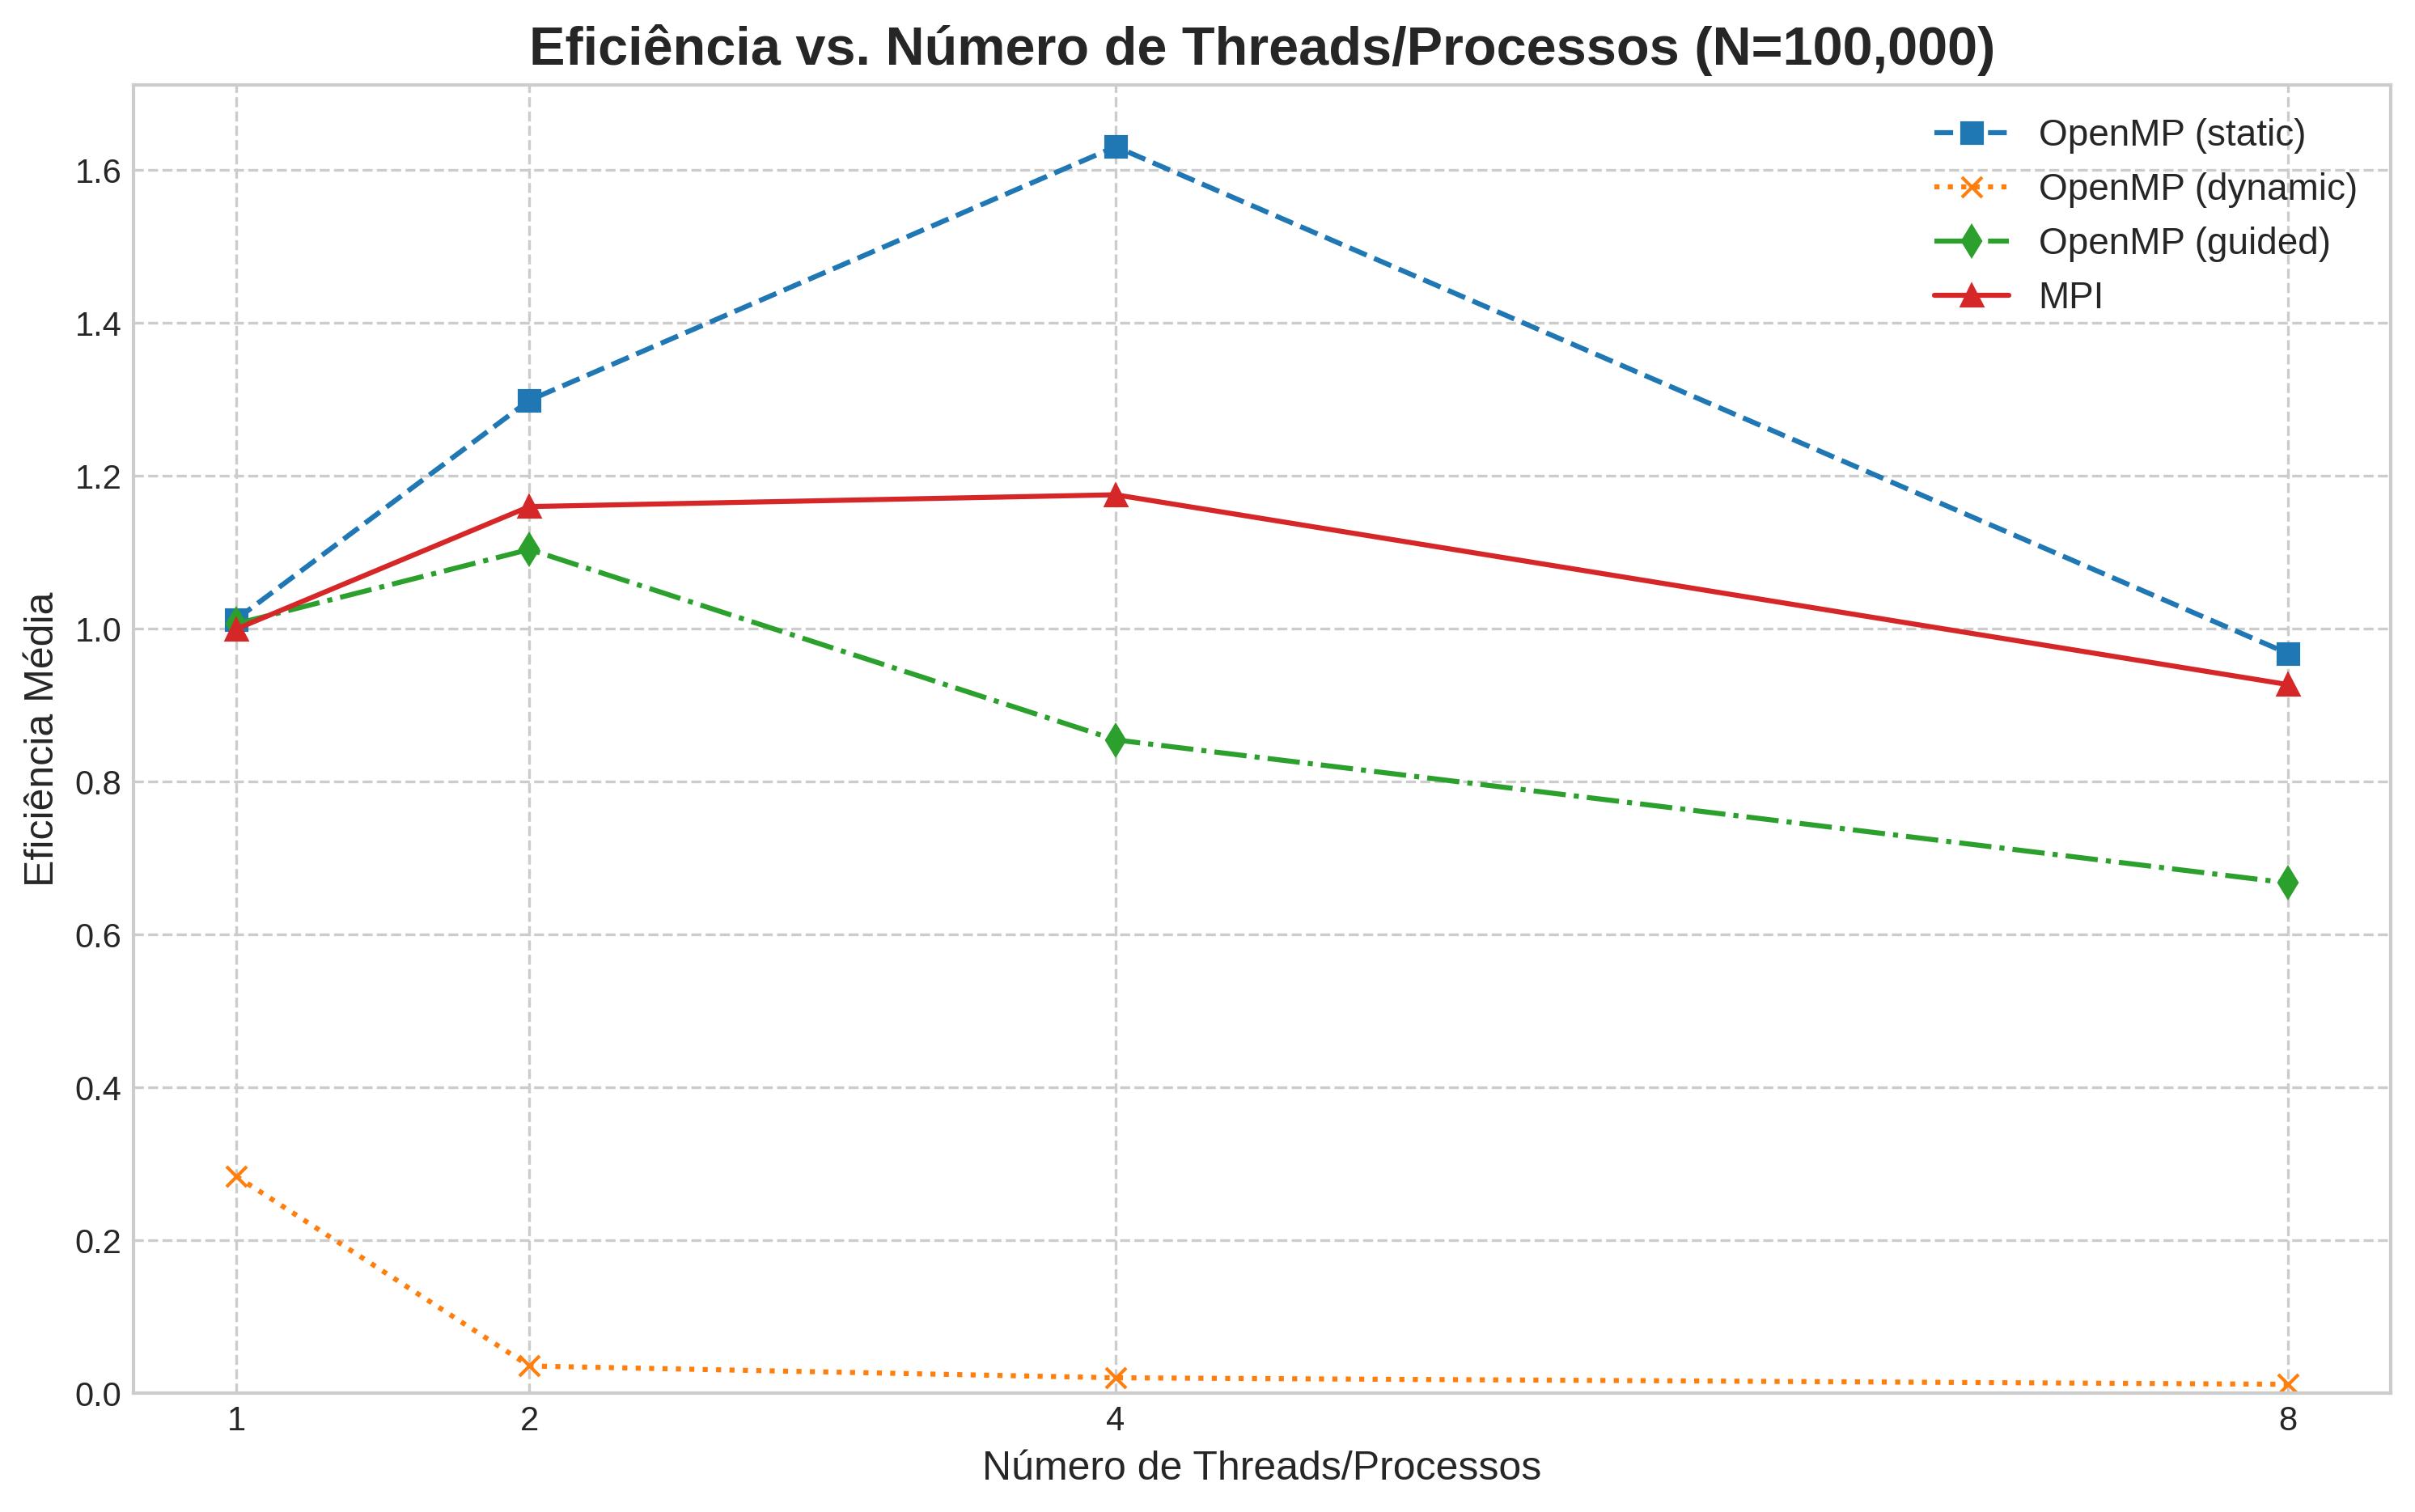
\includegraphics[width=0.9\textwidth]{../graficos/eficiencia_vs_processos_100000.png}
    \caption{Eficiência vs. Número de Processos/Threads ($N=100.000$).}
    \label{fig:eficiencia}
\end{figure}

\section{Discussão e Interpretação dos Resultados}

\paragraph{Análise das Políticas de Agendamento (Scheduling) em OpenMP}
A escolha da política de agendamento em OpenMP revelou-se um fator crítico para o desempenho, como pode ser visto na Tabela \ref{tab:openmp-schedule} e nas Figuras \ref{fig:speedup} e \ref{fig:eficiencia}.
\begin{itemize}
    \item \textbf{Schedule Static:} A política \texttt{static} apresentou o melhor desempenho em todos os cenários. Para um array de 100.000 elementos, alcançou um speedup de 7.74 com 8 threads. Isso ocorre porque o trabalho dentro de cada laço paralelo do Odd-Even Sort é perfeitamente balanceado; cada iteração executa a mesma tarefa (uma comparação e uma possível troca). O agendamento estático, que distribui as iterações de forma equitativa e com baixo custo inicial, é ideal para essa carga de trabalho homogênea.
    
    \item \textbf{Schedule Guided:} A política \texttt{guided} obteve um desempenho intermediário. Embora mais adaptativa que a estática, ela ainda incorre em um overhead maior para gerenciar a distribuição de blocos de iterações, o que não traz benefícios em um cenário de carga balanceada.
    
    \item \textbf{Schedule Dynamic:} A política \texttt{dynamic} mostrou um desempenho drasticamente inferior, sendo mais lenta até que a versão serial (speedup < 1). O alto overhead de alocar cada iteração (ou pequenos blocos) dinamicamente para as threads superou completamente qualquer ganho com a paralelização. Isso demonstra que para problemas com carga de trabalho regular, o custo de gerenciamento do agendamento dinâmico é proibitivo.
\end{itemize}

\paragraph{Análise da Escalabilidade do MPI}
A implementação MPI demonstrou uma forte dependência entre o tamanho do problema e o número de processos. Conforme a Tabela \ref{tab:mpi-all-sizes-filtered}:
\begin{itemize}
    \item Para \textbf{arrays pequenos} (e.g., N=1.000), o desempenho foi fraco, com overhead de comunicação altíssimo (chegando a 90.5\% com 8 processos). O tempo gasto para trocar mensagens entre processos em cada uma das $n$ fases foi maior do que o tempo economizado com a computação paralela.
    
    \item Para \textbf{arrays grandes} (e.g., N=100.000), a implementação MPI mostrou boa escalabilidade, alcançando um speedup de 7.41 com 8 processos. Nesses casos, a quantidade de computação local em cada processo tornou o custo relativo da comunicação muito menor (apenas 33.26\% de overhead com 8 processos). O Gráfico \ref{fig:tempo_vs_tamanho} ilustra claramente que, com 8 processos, a performance do MPI se aproxima muito da melhor versão OpenMP para entradas maiores.
\end{itemize}

\paragraph{Comparativo OpenMP vs. MPI}
Observando as Figuras \ref{fig:speedup} e \ref{fig:eficiencia}, a versão \texttt{OpenMP (static)} consistentemente superou a implementação MPI em speedup e eficiência para N=100.000, embora a diferença diminua com 8 processos. Isso é esperado, pois, em uma máquina de nó único (multi-core), o paradigma de memória compartilhada do OpenMP incorre em um overhead de comunicação muito menor do que a troca de mensagens explícita do MPI.

\paragraph{Eficiência Superior a 100\% (Super-Speedup)}
Um fenômeno notável, visível na Figura \ref{fig:eficiencia} e em ambas as tabelas, é a ocorrência de eficiência maior que 1 (e.g., 1.63 para OpenMP com 4 threads). Isso é conhecido como \textit{super-speedup} e geralmente ocorre devido a efeitos de cache. Quando o problema é dividido, o sub-array alocado para cada thread/processo pode se tornar pequeno o suficiente para caber na cache de nível mais rápido (L1/L2) do processador. A versão serial, ao contrário, processa o array inteiro, potencialmente causando mais falhas de cache (\textit{cache misses}) e acessando a memória RAM, que é mais lenta. O ganho de desempenho ao evitar acessos à RAM pode ser tão significativo que o speedup ultrapassa o número de processadores, resultando em uma eficiência "ideal".

\section{Conclusão}

Este projeto demonstrou com sucesso a paralelização do algoritmo Odd-Even Transposition Sort utilizando os paradigmas de memória compartilhada (OpenMP) e troca de mensagens (MPI). Os resultados confirmaram que a estrutura do algoritmo é altamente propícia à paralelização, mas o desempenho final depende fortemente da implementação, das características da carga de trabalho e do balanço entre computação e comunicação.

A principal conclusão é que, para uma máquina de nó único, a implementação OpenMP com agendamento estático foi a mais eficiente. Isso se deve à natureza regular e balanceada do problema, onde o baixo overhead do compartilhamento de memória e da distribuição estática de tarefas se sobressai. A análise das políticas de agendamento também serviu como um importante lembrete de que a escolha da ferramenta paralela deve ser adequada ao problema.

A implementação MPI, embora menos performática em um único nó devido ao seu overhead de comunicação inerente, mostrou excelente escalabilidade para problemas grandes. Isso indica que seu desempenho seria altamente competitivo e provavelmente superior ao do OpenMP em um ambiente de computação distribuída (cluster), onde a memória não é compartilhada e a troca de mensagens é o único meio de comunicação.

O projeto atingiu seus objetivos, permitindo uma análise prática e quantitativa das métricas de desempenho como speedup, eficiência e overhead. A automação da coleta de dados e geração de gráficos foi fundamental para uma análise sistemática e reprodutível, reforçando as boas práticas em computação de alto desempenho.

\end{document}